%\documentclass[../../Orator]{subfiles}
\documentclass[class={myRUCProject}, crop=false]{standalone}

\usepackage[subpreambles = true]{standalone}
\usepackage{myTikz}

\IfStandalone{%
    \usepackage[disable]{todonotes}
    \import{../../}{customCommands}
    \import{../../}{INP-00-glossary}
    }{}




\begin{document}

%A cell is the basic unit of life, a collection of matter with the ability to perform all the processes necessary for life, including reproducing itself.
%A multi-cellular organism, like humans, is composed of a number of independent cells maintained by complex interactions. How could anyone ever expect these meaty lumps we call `\textit{\glspl{gls:person}}' to coordinate properly without an equally complex system for the transfer of information? 
%\Glspl{gls:neuron} are information highways made manifest in multi-cellular organisms. 
%There exist many distinct types of \glspl{gls:neuron}, however, the underlying mechanisms of function stay the same.
%some of the most important ones are listed below:Of whether they be common skin cells or neuronal, those relevant to this project include the specialized form that neuronal cells have, as well as the ion channels and pumps that allow for the propagation of \gls{ap}, discussed in \Cref{sec:ap}.
%the structures of neuronal cells, and the 
% \subsection{Organelles}



%\section{Relevant Cellular Structures}



% \begin{enumerate}

%     \item \textbf{The Nucleus} is mainly found in the centre of the cell and is responsible for distinguishing between eukaryotic and prokaryotic cells - existing only in the first ones. It functions as the key factor in the cell's activities, it contains most of the cell's genetic information (DNA), and is where the DNA replication, transcription, and RNA processing all happen \cite{organelleDef}.
%     \item \textbf{The Golgi-Apparatus}, an organelle mostly found in eukaryotic cells, transports, modifies, and packages proteins and lipids into vesicles destined for specific intracellular or extracellular locations \cite{organelleDef}. 
%     \item \textbf{The Ribosomes} exist both in eukaryotic and prokaryotic cells. By translating the genetic information from the RNA, they compose proteins and convert genetic code into chains of amino acids. Most ribosomes are found in the endoplasmic reticulum \cite{organelleDef}.
%     \item \textbf{The Endoplasmic Reticulum (ER)} is a cellular organelle that also plays a crutial role in protein and lipid synthesis. There are two types of ER; the rough and the smooth. Rough ER is composed of ribosommes, giving it its rough texture, and makes proteins. In contrast, smooth ER gets its smooth surface because of the lack of ribosomes and is the part of the ER that makes lipids \cite{organelleDef}.
%     \item \textbf{The Mitochondria} are commonly known as the powerhouse of the cell. They are the cell's main source of energy, which they achieve with respiration; the process where glucose and oxygen turn into carbon dioxide and water, releasing energy. Mitochondia also have their own DNA and ribosomes, explaining why not all the genetic information is found in the nucleus \cite{organelleDef}.
%     \item \textbf{The Lysosome} is where the proteins that are not needed anymore end up. It is covered by a membrane and consists of digestive enzymes. Their role is to break down cell parts, like mitochondria, and eliminate invading viruses and bacteria \cite{lysosomeDef}.
  
% \end{enumerate}

\section{Specialized Neuronal Structures}
While sharing resemblances with other types of cells, neurons possess distinct properties that differentiate them from the rest and grant them special features that allow them to perform their selected tasks. One of its unique characteristics is the neuronal structure \cite{lovinger2008communication}. 

%Within a neuron, there is a main cellular area, similar to that of other cells \cite{lovinger2008communication}, also known as the soma. The soma is where the nucleus - the organelle containing genetic material, and other vital cellular organelles reside. %It encompasses the nucleus, a site where the genetic information is transcribed into a single-stranded RNA, particularly the messenger RNA (mRNA) \cite{SHOYKHET2011783}. 
%Furthermore, there is an endoplasmic reticulum (ER) within this region, which is the biggest intracellular organelle \cite{choi2006regional}, containing a set of membranes, responsible for decoding mRNA into a specific sequence of amino acids \cite{SHOYKHET2011783,??}. 
%Additionally, numerous mitochondria are present, contributing to cellular respiration and the synthesis of \gls{atp} \cite{SHOYKHET2011783}. 
%The soma is accompanied by extensions of auxiliary branches - dendrites. These short sprouts receive primarily chemical signals, by means of neurotransmitters, from neighbouring cells through synaptic junctions \cite{lovinger2008communication, SHOYKHET2011783}. 
%Excitatory electrical impulse is then carried through the elongated neural fibre, called the axon \cite{njitacke2020hidden}, and transmitted by means of action potentials, spanning distances of up to several meters \cite{SHOYKHET2011783}.

There exist a number of important structural features that are foundational to the specialized functions found in the \glspl{gls:neuron};
\begin{enumerate}
    \item \glslink{gls:dendrite}{\textbf{The dendrites}} of a \gls{gls:neuron} are extensions of the \gls{gls:membrane} branching from the main body of the neuron - the soma. This overall shape and structure are metaphorically referred to as a `\textit{\gls{gls:denTree}}'\footnotemark~.This is where the majority of \gls{gls:neuron} inputs are received, and carried by the `dendritic spine' down to the \gls{gls:soma}~\cite{Hammond2015ch3,Hammond2015ch4}\footnotetext{Greek root word `\textit{dendron}' meaning tree, translates to `tree tree'.}.
    \item \glslink{gls:soma}{\textbf{The soma}} is the main body of the \gls{gls:neuron}. It is the space in which the nucleus - the organelle containing genetic material, and other vital cellular organelles reside and where protein production occurs. This is mainly where the summation of all the electrical inputs received through the dendrites happens, which will determine whether or not a signal will be fired at the axon hill-lock. (An output signal in neurons is called an action potential.)  %The nucleus can range from \qtyrange{3}{18}{\um} in diameter \cite{Hammond2015ch3,Hammond2015ch4}.
    \item \glslink{gls:axon}{\textbf{The axon}} is a finer tendril that can extend tens, if not tens of thousands, of times the diameter of the \gls{gls:soma} in length. The \gls{gls:axon} primarily carries nerve signals away from the \gls{gls:soma} and carries some types of information back to it. Most \glspl{gls:neuron} have only one \gls{gls:axon}, while others will be able to undergo significant branching, enabling communication with many target cells \cite{Hammond2015ch3,Hammond2015ch4}. 
    \item \glslink{gls:ax-hill}{\textbf{The axon hill-lock}} is the part of the \gls{gls:axon} where it emerges from the \gls{gls:soma}. This region contains the greatest density of voltage-dependent sodium channels, which makes it the most excitable part of the \gls{gls:neuron} and subsequently the site of signal/impulse initiation~\cite{Hammond2015ch3,Hammond2015ch4}. 
    \item \glslink{gls:ax-terminal}{\textbf{The axon terminal}} is found at the terminus of the \gls{gls:axon} \cite{Hammond2015ch3,Hammond2015ch4}. It is the region which establishes connections to other neurons (synapses).
    \item \glslink{gls:myelin}{\textbf{The myelin sheathe}} is a lipid and protein comprised substance excreted from Schwann cells that `sheathes' the \gls{gls:axon}, creating additional insulation for %\gls{gls:capa}~
electrical charge\cite{Hammond2015ch4}.
\end{enumerate}


\begin{figure}[H]
    \centering
    \import{../../Pictures/Anakin}{Neuron.tex}
    \caption{A simplified representation of a \gls{gls:neuron}[al] cell, with labels for each of the important features. (1) the \gls{gls:soma} of the cell; (2) a \gls{gls:dendrite}; (3) the \gls{gls:axon}; (4) the \gls{gls:ax-hill}; (5) the \gls{gls:ax-terminal}.}\label{fig:Neuron}
\end{figure}


%\begin{figure}[H]
 % \centering
  %\import{../../Pictures/Anakin}{Channels.tex}
  %\caption{ $\langle \text{temp, will become channels/pumps} \rangle$ }\label{fig:Channels}
%\end{figure}

\section{Interneuronal communication}

%The nineteenth-century observations by Camillo Golgi and Ramon Cajal on a structure of neurons led to the formulation of two contrasting propositions concerning how neurons communicate with each other. The first working theory was that neurons create netlike structures, resembling the cell arrangement of a heart muscle, thereby establishing a direct transmission of signals through the openings in the neuronal membrane. The second conjecture contended that neurons exist as single cells separated by membranes. The transmission in this case should occur via specific points allowing for chemical signalling between adjacent cells. Although initially in stark opposition, either one has been accurate, and so both means of communication are recognized to contribute to the signal propagation in the brain of mammals \cite{SHOYKHET2011783}.

As was initially suggested by Ramon y Cajal, the information flows from one neuron to the other at points where the axon terminal of one neuron connects to the dendrites of another. These points of contact between neurons that specialize in signal transmission are termed synapses.  The neuron firing the impulse is termed the pre-synaptic neuron, whereas the neuron receiving an input through afferent synapses is called the post-synaptic neuron. Synaptic neuronal communication constitutes a mechanism for rapid impulse transmission \cite{Hammond2015ch6}. 

Cells in the nervous system interact through a mixture of electrical signals (such as electrically charged ions) and chemical signals (e.g., neurotransmitters) \cite{lovinger2008communication} in order to communicate with other cells and and systems \cite{SHOYKHET2011783}. As such, there exist a few types of synapses which include electrical, chemical and mixed type synapses \cite{Hammond2015ch6, SZCZUPAK201699}. 
%Note that synaptic neural communication constitutes a mechanism for rapid impulse transmission. The information is predominately modulated by two classes of synaptic links \cite{SZCZUPAK201699}. Key distinctions between these transmission techniques include the speed of the signal, its accuracy, and that electrical synapses may possibly allow communication in the opposite direction \cite{SZCZUPAK201699}. Yet there are alternative modes of neural transport, thus the communication can occur through mechanisms beyond synaptical scope. Such variants contribute to the overall complexity and adaptability of the nervous system. [??add] 

%All cells in the nervous system interact through the mixture of electrical and chemical signals \cite{lovinger2008communication}, employing a variety of communication strategies, to reach other organs, muscles, and systems \cite{SHOYKHET2011783}. 
%The information is predominately passed via synaptic links, but the communication can also occur through mechanisms beyond the synaptical scope. 
%There are alternative modes of neural transport, such as gap junctions (electrical synapses) or volume transmissions [??]. These variants contribute to the overall complexity and adaptability of the nervous system [??]. 

%\subsubsection{Chemical synapses}
Chemical transmission is made feasible by small distances between the membranes of the connected cells (usually from 20 to 50 nanometres). The space that separates such neurons is called a synaptic cleft. The signal transmission involves a utilization of substances, called neurotransmitters, acting as chemical messengers. They are released by a presynaptic cell (i.e., neuron) into the synaptic cleft. Neurotransmitters bind to specific proteins on the dendritic membrane, known as receptors, which in turn modulate the opening of specific ion channels (gateways of ion flow), which ultimately regulates signal transmission, as will be elaborated further in the paper. In addition to neurotransmitters, there are also other substances, i.e., neuromodulators, hormones, that may not necessarily be released into the synaptic junction but contribute to chemical signal propagation \footnote{This statement is broad enough to include a range of neural cells (etc. glial or endocrine cells) beyond just neurons.} \cite{Hyman2005}.

%\subsubsection*{Electrical Synapses}

In the case of electrical synapses (or gap junctions), the membranes of the connected neurons are in close contact with each other. Here the flow of ions is not regulated by neurotransmitters, ions flow from one cell to the other directly.
%Neurons are in reality mutually isolated due to the presence of external membranes, preventing the direct contact, that would allow them to immediately exchange electrical and chemical signals. Contrary to this case is found within electrical synapses. The protein-based pores, named connexins \cite{sohl2005expression}, facilitates an immediate movement of ions through the closely bounded gap junctions, each of them comprising multiple connexin \footnote{Connexins are not ion channels themselves. They are fundamental compartments of gap junctions, specialized channels facilitating intercellular communication.} channels \cite{SZCZUPAK201699}. They link cytoplasms of two neighbouring neurons, enabling diffusion of ions and small group of atoms (like glucose) among cells \cite{SZCZUPAK201699}, and therefore bypassing the necessity for chemical transmitters \cite{kandel2000principles}. This way, neurons can exchange information regarding their metabolic processes (energy management), and excitability (network dynamics) \cite{SZCZUPAK201699}. Furthermore, myelin structure (sheath) that is generated by glial cells (Schwann cells in PNS, oligodendrocytes \footnote{The predominant subtype of glial cells forming the majority of the human central nervous system \cite{wei2019histology}.} in CNS) connects through gap junctions, producing additional structural support and permitting an immediate diffusion of nutrients in the direction of an axon\cite{SHOYKHET2011783}. Intercellular signal propagation via electrical synapses significantly influences the maturation of the nervous system. It persists, albeit to a lesser extent, in the adult nervous systems of both invertebrates and vertebrates \cite{SZCZUPAK201699} but it is relatively infrequent within the mammalian central nervous system, compared to the chemical transmission \cite{lovinger2008communication, sohl2005expression}. 

Additionally, a synaptic connection may be a combination of an electrical and a chemical synapse. Between neurons in mammals, mixed synapses are more common than the electrical ones \cite{Hammond2015ch6}.
\begin{figure}[H]
    \centering
    \begin{subfigure}[t]{0.25\textwidth}
    \centering
      \caption{}
      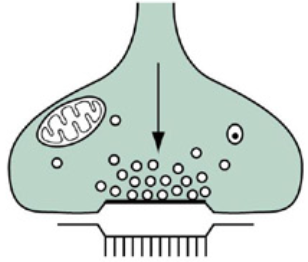
\includegraphics[height=3cm]{Pictures/Anakin/chem.syn.png}
    \end{subfigure}
    \begin{subfigure}[t]{0.3\textwidth}
    \centering
      \caption{}
      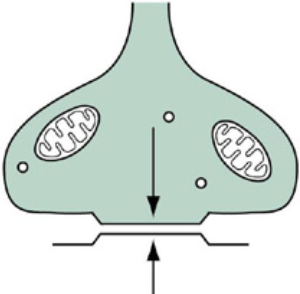
\includegraphics[height=3.3cm]{Pictures/Anakin/el.syn.png}
    \end{subfigure}
     \begin{subfigure}[t]{0.2\textwidth}
    \centering
      \caption{}
      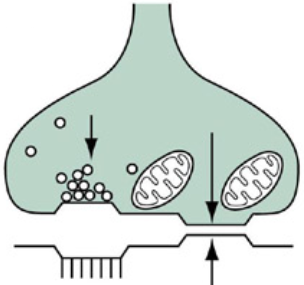
\includegraphics[height=3.2cm]{Pictures/Anakin/mix.syn.png}
    \end{subfigure}
      \caption{Types of synapses. (a) Chemical synapse; (b) electrical synapse (gap junction); (c) mixed synapse. From \cite{Hammond2015ch6}}\label{fig:synapses} 
\end{figure}

\section{The Membrane Potential} 
A fundamental component of cells is the \gls{gls:membrane}, composed of what is known as a `\gls{gls:bilipid}'.{}\footnote{Latin root word `bi' meaning two, translates to `lipid two-layer'} 
A \gls{gls:bilipid} creates a strong electrical insulation, which confers\anakintodo{We need to remember to elaborate} it the property of `\gls{gls:capa}'~\cite{Hammond2015ch3,Hammond2015ch4}.{}\footnote{The capability of an object to store electrical charge.}
In a \gls{gls:neuron}, the overall charge in the \gls{gls:incell} space is more negative relative to the \gls{gls:excell} space. This difference in charge at rest is known as the resting \gls{gls:mPote}, and it is essential for the \gls{gls:neuron}['s] ability to transmit electrical signals \cite{Hammond2015ch3,Hammond2015ch4}. 

By convention, membrane potential - \(\br{\unit{\V\membrane}}\) is the difference between the electric potential of the internal and external faces of the membrane \(\br{\unit{\V\membrane}=\unit{\V\incell}-\unit{\V\excell}}\). In the absence of ongoing electrical activity, this negative potential is termed the resting membrane potential \(\br{\unit{V_{rest}}}\). The usual resting \gls{gls:mPote} is found to be around \glslink{gls:volt}{\qty{-70}{millivolts\br{\milli\volt}}} in \glspl{gls:neuron}, however, it varies depending on the cell type and conditions~\cite{Hammond2015ch3,Hammond2015ch4}. When the membrane potential is less negative than \(V_{rest}\), the membrane is considered to be depolarized. In contrast, when the membrane potential is more negative than \(V_{rest}\), the membrane is said to be \gls{gls:hypol} \cite{Hammond2015ch3}. Depolarization determines excitation, whereas hyperpolarization corresponds to inhibition.

The \glspl{gls:ion} primarily involved in the \gls{gls:mPote} include \gls{Na}, \gls{K}, \gls{Cl} and, to a limited degree, \gls{Ca} (\textbf{\Cref{fig:channels}}). 
In the \gls{gls:excell} space the concentrations of \gls{Na} and \gls{Cl} are kept much higher than in the cytoplasm\kennitodo{perhaps explain?} of the \gls{gls:incell} space, whereas \gls{K} is found in much higher concentrations in the cytoplasm compared to the \gls{gls:excell} space. 
During rest, their concentration \glspl{gls:grad} are actively regulated and maintained at constant values by `\glspl{gls:ionPump}' transporting \glspl{gls:ion} across the \gls{gls:membrane}~\cite{Hammond2015ch3,Hammond2015ch4}. As such, the Na-K-ATPase pump transports 3 \gls{Na} ions out of the cell and 2 \gls{K} ions in the cell for each molecule of ATP (high energy molecule) used.
However, the main contributors to the negative potential of the intracellular side of the \gls{gls:membrane} are the anions of the intracellular fluid, which are organic molecules such as negatively charged amino acids, proteins, nucleic acids, phosphates, etc., which have a large molecular weight and cannot cross the lipid membrane and thus do not participate directly in electrical signaling in neurons~\cite{Hammond2015ch3}. 

%\begin{figure}[H]
 % \centering
  %\import{../../Pictures/Anakin}{Channels.tex}
  %\caption{ $\langle \text{temp, will become channels/pumps} \rangle$ }\label{fig:Channels}
%\end{figure}
\subsection{Ion channels}
An important structure embedded in the \gls{gls:bilipid} includes `\glspl{gls:ionChan}', specialized proteins which permit electrically charged \glspl{gls:ion} to diffuse across the \gls{gls:membrane} \gls{gls:grad}, producing electric current (this will be elaborated in the following sections). Thus, neurons are cells that manifest excitability as their characteristic feature. 

Ion channels are not confined to synapses or dendrites, but are distributed across the whole outer membrane. However, ion channels highly selective and are only permeable to a specific \gls{gls:ion}~\cite{Hammond2015ch4}. Membranes may  contain various types of these channels, like sodium (\gls{Na}), potassium (\gls{K}), calcium (\gls{Ca}), and chlorine (\gls{Cl}), which are all essential for neuron excitability and  (electrical) signal propagation.
\begin{figure}
    \centering
    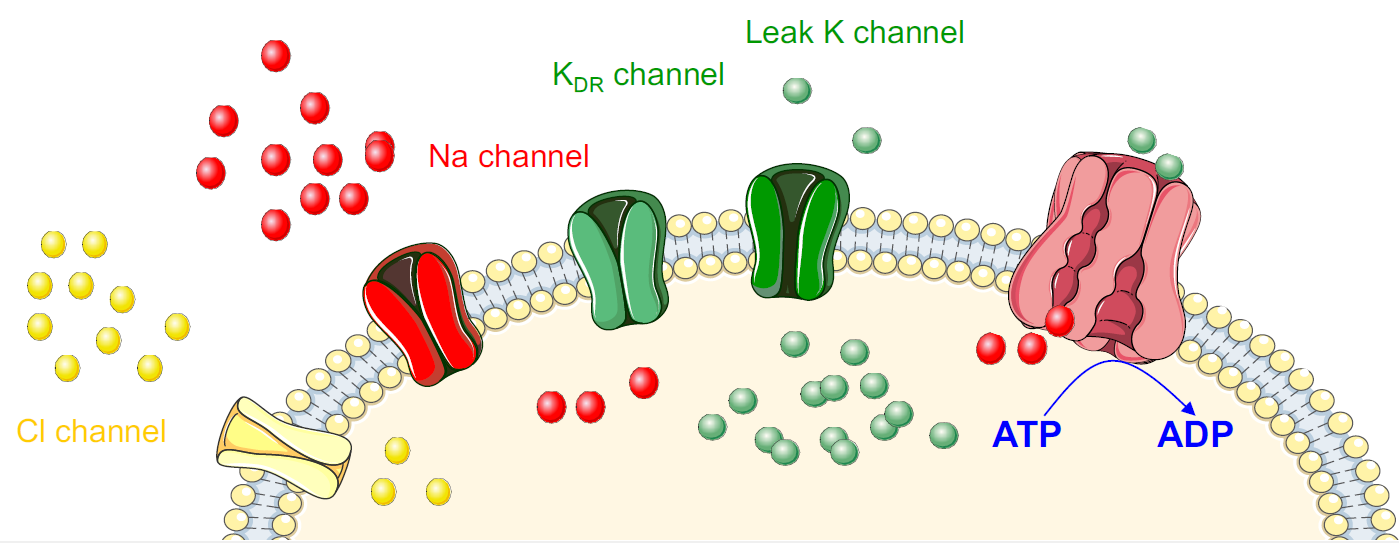
\includegraphics[width=0.75\linewidth]{Pictures//Anakin/channels.png}
    \caption{The structure of the lipid bilayer showing the relative concentrations of the ions as well as their respective ion channels and the Na-K-ATPase pump. \cite{channels}}
    \label{fig:channels}
\end{figure}

Some \glspl{gls:ionChan} are \gls{gls:vgate}[d], meaning that they can be switched between open and closed states in response to changes in the voltage across the \gls{gls:membrane}. 
Others are `\gls{gls:lig} gated', meaning that they  open upon binding of certain molecules (\gls{gls:lig}s) like neurotransmitters, released into the synaptic cleft by the presynaptic neuron. The coupling of neurotransmitters to receptors on a postsynaptic dendritic membrane initiates a reaction in a postsynaptic cell, which leads to either depolarization (excitation) or hyperpolarization (inhibition). The outcome is contingent on the class of the neurotransmitter, the specific protein – receptor interaction, and the neuronal circuitry.

%The overall concept of ion channels is unique to the field of biology and neuroscience. The terminology may vary based on the field, meaning that in the context of physics or materials science one may write about the electron or proton channels instead, when discussing the passage of charged particles.

%Ion channels are highly selective, they permit the transition of only a certain class of charged particles – as the name suggests, ions. 
%they are implicitly designed to accommodate the flow of specific ions, dependent upon the channel’s characteristics. 
%Membranes may  contain various types of these channels,  like sodium (Na+), potassium (K+), calcium (Ca2+), and chloride (Cl-), which are essential for the (electrical) signal propagation including action potentials, excitability of a neuron, and some other cell functions.

%The movement of ions and the channel selectivity is often determined by the size and charge of the specific atom they transport. 
%But one can also say this the other way round. The structure of an ion channel comprises a pore through which ions traverse and so that the dimensions and shape of the pore dictates exactly which ion is permitted to go through, excluding every other. 
% For other charged particles, such as electrons or protons, even though they are notably smaller and distinctly charged, neither one of them is commonly transported through ion channels, since these types of atoms are beyond the scope of biological systems. 

\vspace{1em}




\subsection{Ions Diffuse Downstream of Their Electrochemical Gradient}

% Passive vs facilitated diffusion

The direction of the diffusion of \glspl{gls:ion} through an open channel depends on both the concentration \gls{gls:grad} of the \gls{gls:ion} and the \gls{gls:mPote}. The resulting combination of these two forces is called the electrochemical \gls{gls:grad} \cite{Hammond2015ch3}.
% \begin{align}
%     J_m + D\ode{c} =& 0\\
%     J_e + \sigma\ode{E} =& 0\\
%     \implies \br{J_m + J_e} + \br{D\ode{c} + \sigma\ode{E}} =& 0
% \end{align}



For instance, when the \gls{gls:mPote} is null \(\br{\unit{\V\membrane}=\qty{0}{\mV}}\), there is no difference of \gls{gls:Pote} between the two faces of the \gls{gls:membrane}, so the concentration \gls{gls:grad} will be the only factor determining the direction of diffusion for specific \glspl{gls:ion}. 
Since the concentrations of \gls{Na}, \gls{Ca} and \gls{Cl} in the \gls{gls:excell} fluid are higher, on average, than in the \gls{gls:incell} medium, these \glspl{gls:ion} will diffuse passively towards the \gls{gls:incell} space,\footnote{via \gls{Na}, \gls{Ca} or \gls{Cl} permeable ion channels}~as a result of their concentration \gls{gls:grad}. 
In contrast, since \gls{K} is a lot more abundant in the intracellular \gls{gls:media}, it will move from the \gls{gls:incell} \gls{gls:media} to the \gls{gls:excell} one when \gls{K} permeable channels are open\cite{Hammond2015ch3}. 

If we suppose that there is the same concentration of each \gls{gls:ion} in the \gls{gls:excell} and \gls{gls:incell} \glspl{gls:media}, i.e there is no concentration \gls{gls:grad} for any \glspl{gls:ion}, \glspl{gls:ion} will diffuse according to \gls{gls:mPote} only: positive ions (cations) will move towards negative potential, negative ions (anions) will move towards postive \gls{gls:Pote}. At a \gls{gls:mPote} \(\unit{\V\membrane}=\qty{-30}{\mV}\), positively charged \glspl{gls:ion}, the \glspl{gls:cation} \gls{Na}, \gls{Ca} and \gls{K}, will move from the \gls{gls:excell} \gls{gls:media} to the \gls{gls:incell} one according to \gls{gls:mPote}. In contrast, \glspl{gls:anion} (\gls{Cl}) will move from the \gls{gls:incell} \gls{gls:media} to the \gls{gls:excell} one \cite{Hammond2015ch3}. 

%In physiological conditions, both the concentration \gls{gls:grad} and \gls{gls:mPote} determine the direction and amplitude of \gls{gls:ion} diffusion through an open channel.
In physiological conditions, the concentration \gls{gls:grad} is maintained constant for each \gls{gls:ion}, so the direction and amplitude of diffusion mainly varies with \gls{gls:mPote}. 
%When comparing \Cref{sfig:dirA,sfig:dirB} it appears that the concentration \gls{gls:grad} and the \gls{gls:mPote} (at \(\qty{-30}{\mV}\)) drive \gls{Na} and \gls{Ca} \glspl{gls:ion} in the same direction, toward the \gls{gls:incell} \gls{gls:media}, whereas the direction that \gls{K} and \gls{Cl} ions are driven is reversed . 
The resultant of these two potentials, concentration and \gls{gls:Pote} \glspl{gls:grad}, is the electrochemical \gls{gls:grad}. To know how to express the electrochemical \gls{gls:grad}, the \gls{gls:ePote} must first be explained.
 
% \begin{figure}[H]
%     \nextfloat
%   \begin{subfigure}[t]{0.45\textwidth}
%     \centering
%     \caption{}\label{sfig:dirA}
%     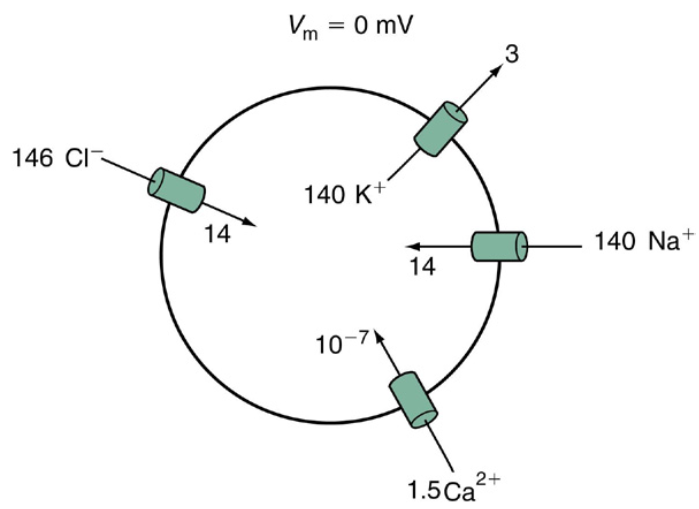
\includegraphics[height=6cm]{Pictures/Anakin/c.grad.png}
%   \end{subfigure}
%   \hfill
%   \begin{subfigure}[t]{0.45\textwidth}
%     \centering
%     \caption{}\label{sfig:dirB}
%     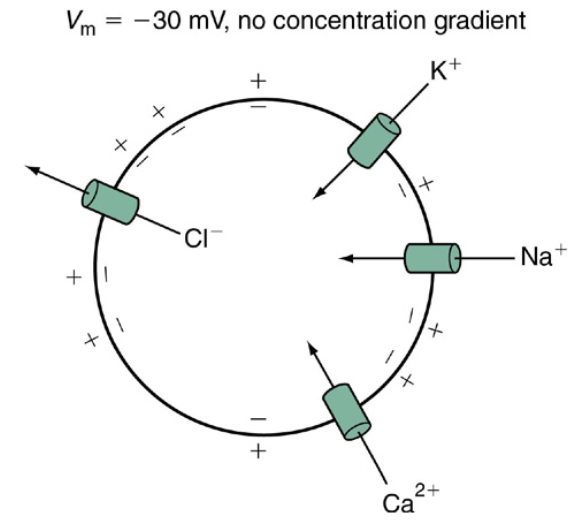
\includegraphics[height=6cm]{Pictures/Anakin/el.grad.png}
%   \end{subfigure}
%     \caption{Passive diffusion of \glspl{gls:ion}. Passive diffusion of \glspl{gls:ion} according \labelcref{sfig:dirA} their concentration \gls{gls:grad} only, or \labelcref{sfig:dirB} to \gls{gls:membrane} \gls{gls:Pote} (electrical \gls{gls:grad}) only \(\br{\unit{\V\membrane} = \qty{-30}{\mV}}\). From \cite{Hammond2015ch3}.}\label{fig:direction} 
% \end{figure}
\subsection{Equilibrium Potential of a Given Ion}
\begingroup
\allowdisplaybreaks
All systems yearn for their \gls{gls:equil}, the fabled \textit{steady state}. This divine relation of the components in a system, one achieved, the system no longer needs to evolve, it has been perfected by \gls{gls:entropy}.
The value of the \gls{gls:mPote} is constantly fluctuating depending on the relative distribution of charged particles that cross the \gls{gls:membrane}.
% The relationship can be illustrated as the relative `work' \(\br{W}\) of concentrations, where  \(\br{W_c}\) represents the potential moving against the electrical gradient done by the concentration gradient, and \(\br{W_e}\) is the potential of the electrical gradient against concentration. The equilibrium exists at;
% \begin{equation}
%     W_e + W_c = 0
% \end{equation}
%The \gls{gls:ePote} for a particular \gls{gls:ion} is the value of \(\unit{\V\membrane}\) for which the net \gls{gls:flux} of this \gls{gls:ion}\(\br{f_\bfm{net}}\) through an open channel is null: when \(\unit{\V\membrane} = \equi\ion\), \(f_\bfm{net} = \qty{0}{\mole\per\second}\).
When the \glspl{gls:grad} are balanced at net zero, it is referred to as the `\gls{gls:ePote}' of the given \gls{gls:ion} \br{\equi\ion}, alternatively, as the `\gls{gls:rPote}' of the \gls{gls:ion} \(\equi\reverse\). 
The \(\equi\ion\) of the given \glspl{gls:ion} can be calculated using the \emph{Nernst} equation for equilibrium potential of an ion species:
\begin{subequations}\label{eq:nernst}
\begin{equation}
  \equi\ion = \br{\frac{\clm{R}\, \cdot \,\clm{T}}{z\, \cdot \, \clm{F}}} \, \ln \br{\frac{\ionconc\excell }{ \ionconc\incell} } \tag{\ref*{eq:nernst}} 
\end{equation}
Where \(\clm{R}\) is the ideal gas constant \br{\qty{8.314}{\cubic\meter\pascal\per\kelvin\per\mol}}; \(\clm{T}\) is the temperature in \gls{gls:kelvin} \(\br{ x\,\unit{\glssymbol{gls:celsius}} \cong {273.15} + x\,\unit{\kelvin}}\); \(\clm{F}\) is the Faraday constant \br{\qty{96500}{\coulomb\per\mole}}; \(z\) is the valence of the \gls{gls:ion}; and \(\ionconc\) is the concentration of the given \gls{gls:ion} in the \gls{gls:excell} \( \br{ \clm{E} } \) or \gls{gls:incell} \( \br{\clm{I}}\) \gls{gls:media}. 
% As most of these terms are constants, it is simple to reduce the equation down in dimensional complexity:
% \begin{align} 
%     \equi\ion &= \br{\frac{ \qty{8.314}{\cubic\meter\pascal\per\mol\per\kelvin} \, \cdot \, \clm{T}}{ z\, \cdot \, \qty{96500}{\coulomb\per\mole} }} \,\ln \br{ \frac{ {\ionconc\excell} }{ {\ionconc\incell}} } \\
%     \intertext{dividing and rearranging the terms:}
%     \equi\ion &= \br{\frac{ \clm{T}\unit{\per\K} \, \unit{\cubic\meter\pascal} }{ z\, \cdot \, \qty{11612.515042118}{\coulomb} } } \cdot \,\ln \br{ \frac{ {\ionconc\excell} }{ {\ionconc\incell}} } \\
%     %
%     \intertext{converting the unit of pressure, pascal \br{\unit{\pascal}} to the base units representing mass over an area over time \br{\unit{\kilo\gram\per\meter\per\square\second}}, as well converting the unit for charge, a \gls{gls:coulomb} \br{\unit{\coulomb}}, to the base units denoting the quantity of current in a second, \br{\unit{\ampere\second}}, gives the substitution:}
%     \equi\ion &= \br{\frac{ \clm{T}\unit{\per\K} \, \unit{\cubic\meter\kilo\gram\per\meter\per\square\second} }{ z\, \cdot \, \qty{11612.515042118}{\ampere\second} } } \cdot \,\ln \br{ \frac{ {\ionconc\excell} }{ {\ionconc\incell}} } \\
%     \intertext{a unit which is equivalent to a Volt, \( \unit{\volt} = \unit{\kilo\gram\square\meter\per\cubic\second\per\ampere} \), the combination of units found through deconstruction is the literal base unit definition of a volt:}
%     \equi\ion &= \frac{ \clm{T}\unit{\per\K} }{ z\, \cdot \, \num{11612.515042118}} \cdot \unit{\volt} \cdot \ln \br{ \frac{ {\ionconc\excell} }{ {\ionconc\incell}} }\label{eq:derivedNerst}
% \end{align}
%{Volume Concentration \per\kelvin\per\mol}
%{\kilo\gram\metre^2\second^{-2}\kelvin\per\mol}
\end{subequations}

\begin{subequations}\label{eq:mVions}
With minor adjustments\footnote{Left as an exercise for the reader} to \cref{eq:nernst}, % the now derived form of \cref{eq:nernst}, 
one is able to derive;
\begin{equation}
  \equi\ion = \cfrac{\clm{T}\unit{\per\K}}{ z } \, \cdot \, \ln \br{ \frac{ {\ionconc\excell} }{ {\ionconc\incell}} } \cdot \num{11.612515042}^{-1} \ \unit{\milli\volt} \tag{\ref*{eq:mVions}}
\end{equation}

Plugging the relative concentrations, measured in millimoles \br{\unit{\milli\mol}}, of each \gls{gls:ion} into \cref{eq:mVions}, as well as choosing an arbitrary temperature, such as human body temperature \(\approx\) \qty{37}{\degreeCelsius} \(\br{\sbr{\num{37} + \num{273.15}}\unit{\glssymbol{gls:kelvin}}}\),
using the relevant \(\ionconc\),
the \glspl{gls:ePote} follow:

\noindent
\scalebox{0.90}{
\begin{minipage}[c]{.525\textwidth}
  \begin{align}
    {\equi\sodium} &= \num{310.15}\ \ln \br{ \frac{142}{15} }\cdot \num{11.612515042}^{-1} &=& \qty{60.034194963}{\mV} \label{eq:Na}\\
    {\equi\potassium} &= \num{310.15}\ \ln \br{ \frac{4}{150} }\cdot \num{11.612515042}^{-1} &=& \qty{-96.799817808}{\mV} \label{eq:K}
    \end{align}
\end{minipage}}
\hfill
\scalebox{0.90}{
\begin{minipage}[c]{.525\textwidth}
  \begin{align}
    {\equi\chlorine} &= \num{-310.15}\ \ln \br{ \frac{120}{\num{5}} }\cdot \num{11.612515042}^{-1} &=& \qty{-90.840043187}{\mV} \label{eq:Cl}\\
    {\equi\calcium}  &= \frac{310.15}{2}\ \ln \br{ \frac{1}{\num{e-4}} }\cdot \num{11.612515042}^{-1} &=& \qty{122.996054517}{\mV} \label{eq:Ca}
  \end{align}
\end{minipage}}

% 293.15

% 58.127185848 
% -97.014667339
% 121.372216367
% -59.186543354

\end{subequations}

\endgroup



\subsection{Ionic currents}
The passive diffusion of \glspl{gls:ion} through an open channel implies a movement of charge through some resistance. Current comes from the movement of charge.
When focusing on a single channel, the current is called `single-channel current' or `unitary current', \(\br{\ucur\ion}\). The amplitude of \(\ucur\ion\) is expressed in ampere \(\br{\unit{\ampere}}\) which are coulombs per seconds \(\br{\unit{\coulomb\per\second}}\) \cite{Hammond2015ch3}. 

In general, currents are expressed following Ohm's law: \(\rmm{U}=\rmm{Z}\curr\), where \(\curr\) is the current through a resistance \(\rmm{Z}\) and \(\rmm{U}\) is the difference of \gls{gls:Pote} between the two ends of the resistance. 
For currents created by \gls{gls:ion}[ic] charge (and not by electrons as in copper wires), \(\curr\) is labeled \(\curr\ion\), the current that passes through the resistance of the channel pore which has a resistance \(\rmm{R}\) \(\br{\res\ion}\) \cite{Hammond2015ch3}. 
%
But what is \(\rmm{U}\) in biological systems? 
%
\unit{U} is the electrical potential, directing the \glspl{gls:ion} along a particular axis; it is the electrochemical \gls{gls:grad} for the considered \gls{gls:ion} and is also called the driving potential: \(\rmm{U}=(\unit{\V} - \equi\ion)\). According to ohm's law, the current \(\curr\ion\) through a single channel is derived from 
\begin{equation}
  \unit{\V} - \equi\ion = r\ion \cdot \curr\ion
\end{equation}
So:
\begin{equation}\label{eq:cur2con}
  \curr\ion= \frac{1}{r\ion\br{\unit{\V} - \equi\ion}} = \ucon\ion(\unit{\V\membrane} - \equi\ion)
\end{equation}
%\(\ucon\ion\) 
The measure of the \glspl{gls:ion} through a single channel, is called the unitary \gls{gls:contan} \(\br{\ucon\ion}\) which is the real part of \gls{gls:admit} \cite{Hammond2015ch3}. 
The reciprocal of resistance; it is called the \textit{\gls{gls:admit}}.
While resistance is expressed in \gls{gls:ohm} \(\br{\unit{\ohm}}\), \gls{gls:admit} is expressed in siemens \(\br{\unit{\siemens}}\).\footnote{\Gls{gls:admit} can also be expressed in `mho' which is inverse ohm, \(\unit{\ohm}^{-1} = \unit{\mho}\)}~
By convention \(\curr\ion\) is negative when it represents an inward \gls{gls:flux} of positive charges (\glspl{gls:cation}) and \(\curr\ion\) is positive when it represents an outward \gls{gls:flux} of positive charges. It is generally of the order of pico-ampere \(\br{\qty{1}{\pico\ampere}=\qty{e-12}{\ampere}}\). At physiological concentrations, \(\ucon\ion\) varies between \(\qtyrange{10}{150}{\pico\siemens}\) dependent on channel type~\cite{Hammond2015ch4}.

\(\curr\ion\) and \(\ucur\ion\) can be measured experimentally. 

{}\(\curr\ion\) is current measured from a whole \gls{gls:membrane} where \(N\) channels of the same type are present. \(\ucur\ion\) is measured current from a patch of \gls{gls:membrane} where only one channel of a given type is present.The techniques mainly used for measuring ionic currents in excitable cells are the current- and voltage- clamp techniques \cite{Hammond2015ch4}.

\subsubsection{Current clamp}\label{sec:Cclamp}
% \anakintodo{appendix?}

Current clamping is a technique for recording the membrane potential and how that potential changes by injecting current into a cell through the recording \gls{gls:electrode}.  
`Current clamp' implies that the current applied through the electrode is held at a constant value for the experiment, while the membrane potential is free to vary~\cite{Hammond2015ch4}. The amplifier records whatever voltage the cell generates on its own or as a result of stimulation. 
This technique is useful for studying how a cell responds when electric current enters a cell~\cite{Hammond2015ch4}.

\subsubsection{Voltage clamp technique}\label{sec:Vclamp}
% \anakintodo{appendix?} 
 
In contrast to the current clamp technique, in voltage clamp mode the cell membrane potential is `clamped' at a chosen value while changes in ionic currents are recorded ~\cite{Hammond2015ch4}. 
This allows to measure how much \textit{ionic current} is flowing through the cell's membrane at any given voltage. 
This is important because, as will be elaborated in \Cref{sec:depol}, many of the ion channels in neuronal membrane are \gls{gls:vgate}[d] ion channels, which open only when the membrane voltage is within a certain range, and the voltage clamp technique allows for control of the variable determining the opening of those channels~\cite{Hammond2015ch4}. It controls the voltage across the membrane to a specific value so that the behavior of system in study is independent of it. Originally, this experiment was done on a squid axon since it was relatively larger than most and would allow for less intricate experimental setups.

The key components of the setup are the following:

\textbf{ Reference electrode:} Compares the voltage with the one inside in order to measure the voltage difference.

\textbf{ Command voltage:} The desirable voltage that is controlled by a diode that can drop the voltage according to the voltage difference. This will generate a current that will be injected back to the system. Such current will balance the voltage to the desirable one.

\textbf{ Measured current:} Current needed to keep the voltage the same as the command voltage. How the needs to vary in accordance to the ion channels will give insight into how the channels work(conductance for example).

\begin{figure}[H]
    \centering
    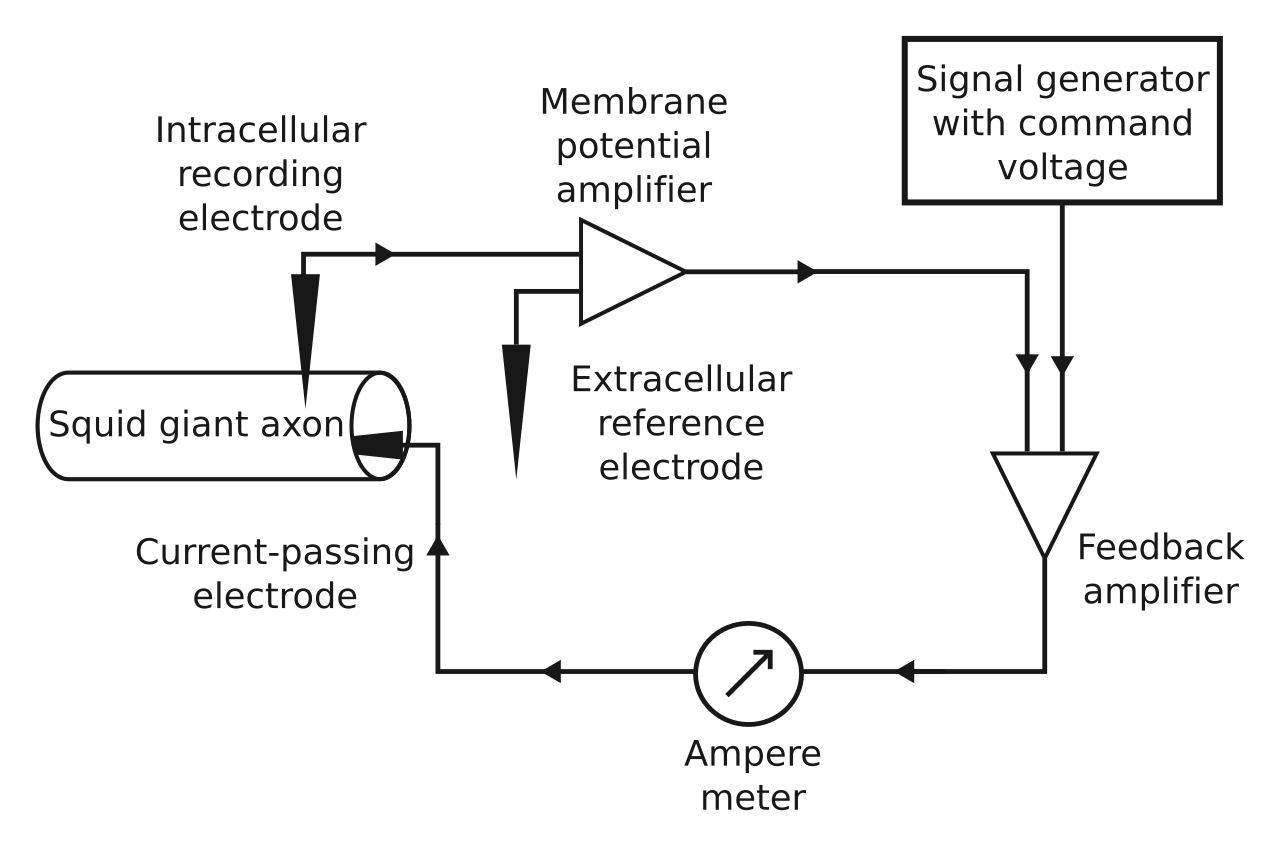
\includegraphics[width=0.55\textwidth]{Pictures/Anakin/Vclamp.png}
    \caption{The voltage clamp setup of a squid giant axon.}\label{fig:Vclamp}
\end{figure} 

A variation of  voltage clamp technique is the patch clamp technique, which allows to isolate currents from patches of cell membrane or even individual ion channels~\cite{Hammond2015ch4}.%(unitary currents \(\ucur\ion\))

\section{The Action Potential}\label{sec:ap}



%An \gls{ap} occurs when the \gls{gls:Pote} of an excitable cell's \gls{gls:membrane} rapidly rises and falls. This \gls{gls:depol} then causes adjacent regions to similarly `depolarize', creating a chain reaction in the form of a `wavelet'.
%The voltage fluctuations take the form of a rapid upward spike followed by a rapid fall.

%``All-or-none'' principle


\begin{comment}
  Each excitable patch of \gls{gls:membrane} has two important levels of \gls{gls:mPote}: the resting potential, which is the value the \gls{gls:mPote} maintains as long as nothing perturbs the cell, and a higher value called the \gls{gls:tPote}. At the axon hillock of a typical \gls{gls:neuron}, the resting \gls{gls:Pote} is around –70 millivolts (mV) and the threshold \gls{gls:Pote} is around –55 mV. Synaptic inputs to a \gls{gls:neuron} cause the \gls{gls:membrane} to depolarize or hyperpolarize; that is, they cause the \gls{gls:mPote} to rise or fall. \glspl{ap} are triggered when enough \gls{gls:depol} accumulates to bring the \gls{gls:mPote} up to threshold. When an \gls{ap} is triggered, the \gls{gls:mPote} abruptly shoots upward and then equally abruptly shoots back downward, often ending below the resting level, where it remains for some period of time. The shape of the \gls{ap} is stereotyped; this means that the rise and fall usually have approximately the same amplitude and time course for all \glspl{ap} in a given cell. (Exceptions are discussed later in the article). In most \glspl{gls:neuron}, the entire process takes place in about a thousandth of a second. Many types of \glspl{gls:neuron} emit \glspl{ap} constantly at rates of up to 10–100 per second. However, some types are much quieter, and may go for minutes or longer without emitting any \glspl{ap}.

  \glspl{ap} result from the presence in a cell's \gls{gls:membrane} of special types of \gls{gls:vgate}[d] \glspl{gls:ionChan}.[6] A \gls{gls:vgate}[d] \gls{gls:ion}channel is a transmembrane protein that has three key properties:

  It is capable of assuming more than one conformation.
  At least one of the conformations creates a channel through the \gls{gls:membrane} that is permeable to specific types of \glspl{gls:ion}.
  The transition between conformations is influenced by the \gls{gls:mPote}.
  Thus, a \gls{gls:vgate}[d] \gls{gls:ion}channel tends to be open for some values of the \gls{gls:mPote}, and closed for others. In most cases, however, the relationship between \gls{gls:mPote} and channel state is probabilistic and involves a time delay. \Glspl{gls:ionChan} switch between conformations at unpredictable times: The \gls{gls:mPote} determines the rate of transitions and the probability per unit time of each type of transition.
\end{comment}
%original text
As mentioned earlier, activation of afferent synapses generates excitatory or inhibitory currents on the synaptic membrane of the post-synaptic neuron through receptor channel activation by neurotransmitters. The resulting postsynaptic currents travel along dendrites towards the soma and to the axon initial segment in the postsynaptic neuron. During the course of their propagation, these currents summate. If their cumulative effect achieves enough membrane depolarization at the axon initial segment, a post-synaptic response will be triggered. This post-synaptic response is the  \gls{ap} -  a sudden and rapid \gls{gls:depol} of the \gls{gls:membrane} propagating along the length of the axon towards the axon terminal, where it will result in the release of neurotransmitters. AP is the result of opening of voltage-gated \gls{Na} channels at the axon hillock, where they are most abundant \cite{Hammond2015ch13}. 


Up to a threshold level of \gls{gls:membrane} \gls{gls:depol} (called the \gls{gls:tPote}), only passive ohmic response can be recorded, when the \gls{gls:membrane} is depolarized just above the threshold, an \gls{ap} is evoked. \anakintodo{Include section about number of subunits in squid channels}
Increasing the intensity of the stimulating current pulse does not increase the amplitude of the \gls{ap}, the \gls{ap} is all or none \cite{Hammond2015ch4,kandel2000principles}. 

The way the action potential travels along the axon is much like a flame moving along a fuse \cite{wood1996neuroscience}. The flow of the positive charge extends through the axon causing a further depolarization of neighboring segments when they too, reach the threshold value. Consequentially, the \gls{gls:flux} of \gls{Na} \glspl{gls:ion} increases, causing further \gls{gls:depol} of the \gls{gls:membrane}, cascading until all \gls{Na} channels in the segment have opened.  This coincides with the \gls{gls:depol} phase reaching its peak \cite{Hammond2015ch4}.  

This propagation proceeds without \gls{gls:attenuation} due to the density of \gls{gls:vgate}[d] \gls{Na} channels remains constant along the axon; as well due to the presence of insulating \glspl{gls:myelin}.  In this manner, the  \gls{ap} travels down the axon until it reaches the terminal, commencing interneuronal communication \cite{wood1996neuroscience}. The time during which the \gls{Na} channel stays open is the mean open time, denoted \(\tau_o\) \cite{Hammond2015ch4}\footnote{The letter  `o', not the number `0'} and once they inactivate they may not reopen, which guarantees the unidirectional propagation of the action potential \cite{Hammond2015ch4}. 
%Similar to the fuse scenario, the signal might initiate from both tails of the axon upon depolarization, allowing for bidirectional transmission \cite{wood1996neuroscience}.

\begin{figure}[H]
  \centering
  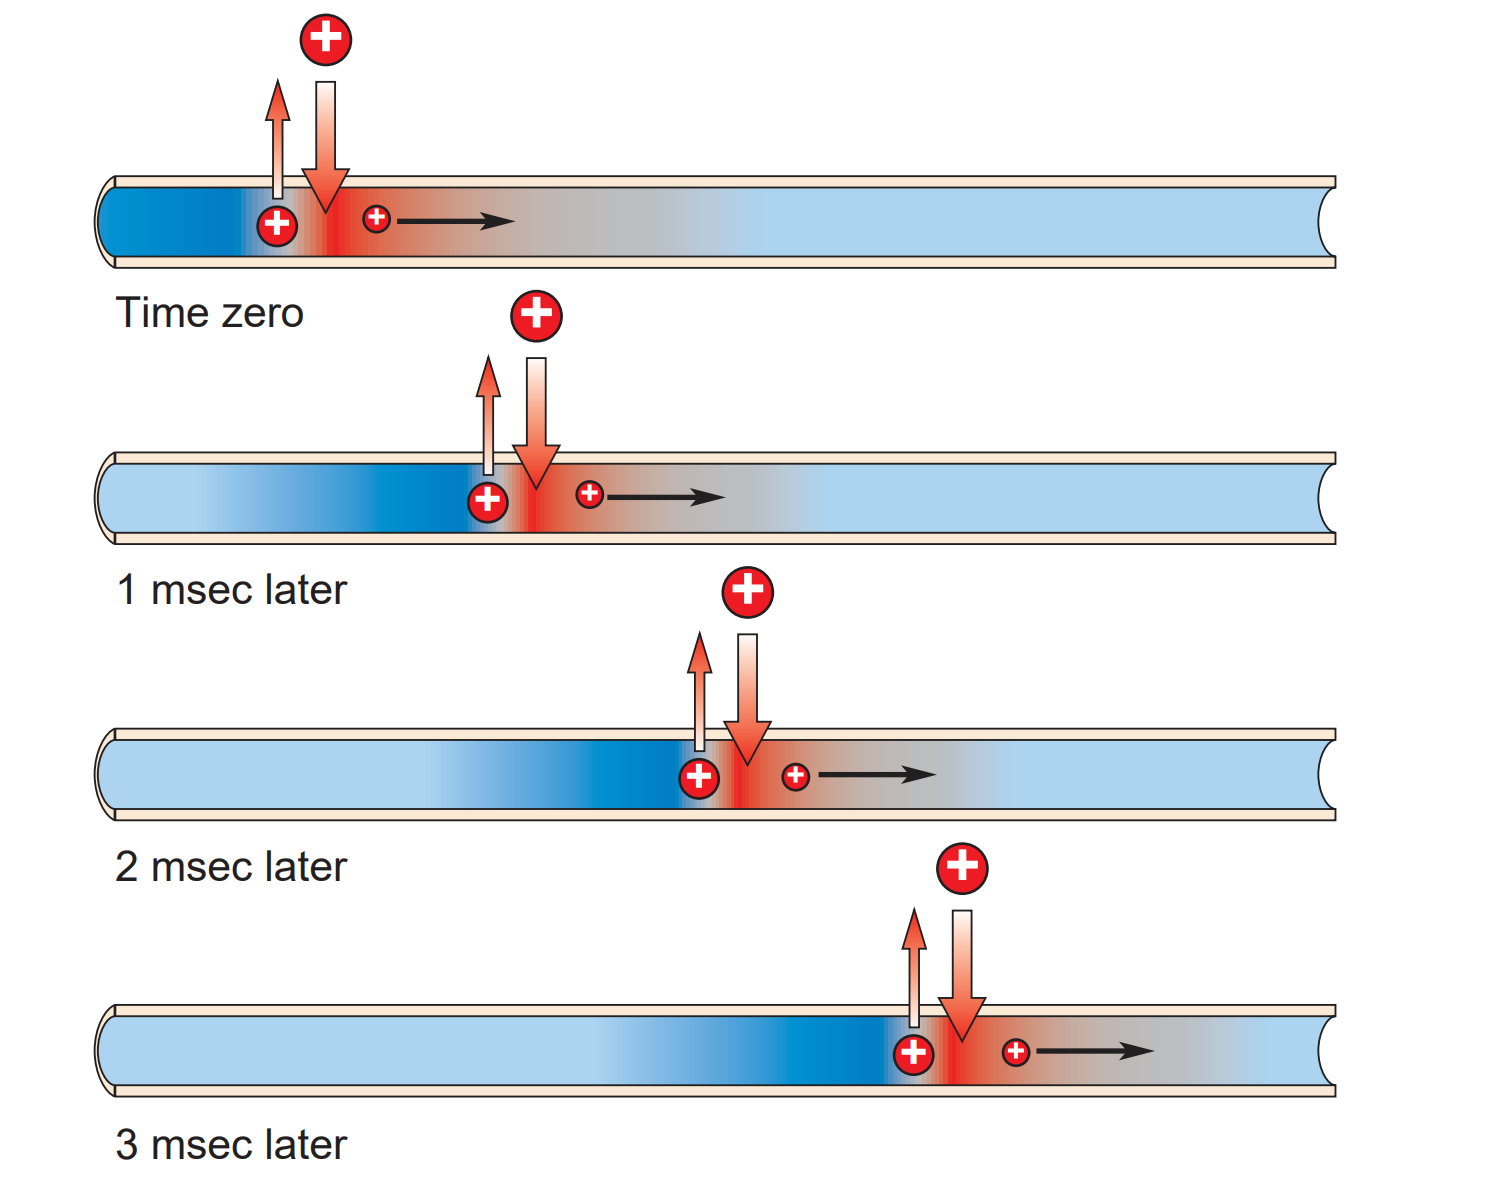
\includegraphics[width=0.4\linewidth]{Pictures/Svet/Screenshot (903).png}
  \caption{\textbf{Signal propagation in the axon segment.} The action potential's positive charge influx prompts the membrane in front to depolarize by reaching the threshold \cite{wood1996neuroscience}.}\label{fig:cond}
\end{figure}

\subsection{The ionic dynamics underlying APs}

The \gls{gls:ion}[ic] basis for \gls{gls:neuron}[al] excitation was first described in the giant squid axon by Hodgkin \& Huxley \br{1952} using the voltage clamp technique~\cite{HodHux1952}.\footnote{\cref{sec:Vclamp}}{} They observed a key phenomenon, that the \gls{ap} is underlied by two separate voltage-dependent currents: an early transient inward \gls{Na} current which depolarizes the \gls{gls:membrane}, and a delayed outward \gls{K} current largely responsible for \gls{gls:repol}. 
The resulting voltage waveform takes the shape of a rapid upward spike followed by a rapid inactivation that hyperpolarizes the \gls{gls:membrane} before returning to the resting \gls{gls:mPote} \cref{fig:AP} \cite{Hammond2015ch4}.
%\begin{figure}[H]
%  \centering
 % 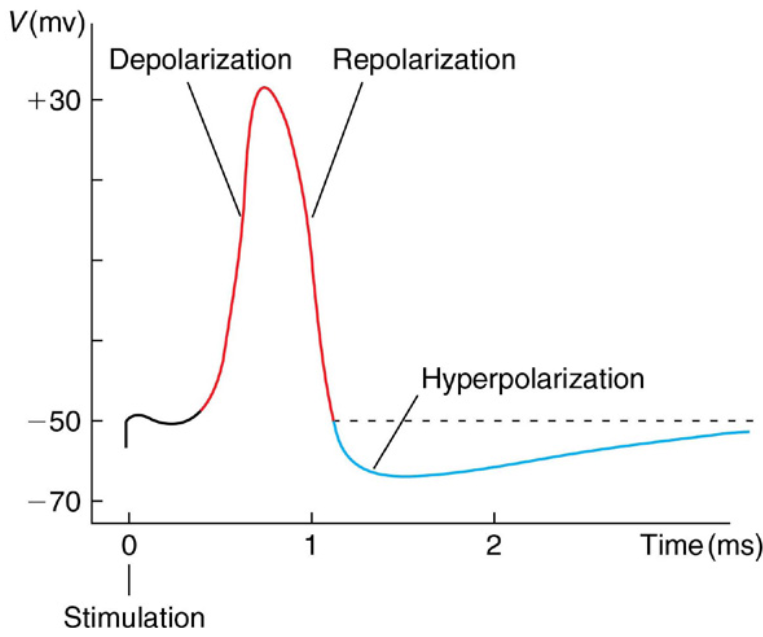
\includegraphics[width=0.5\linewidth]{Pictures//Anakin/AP.png}
  %\caption{The action potential spike, indicating the different phases.}\label{fig:AP}
%\end{figure}

\begin{figure}[H]
  \centering
  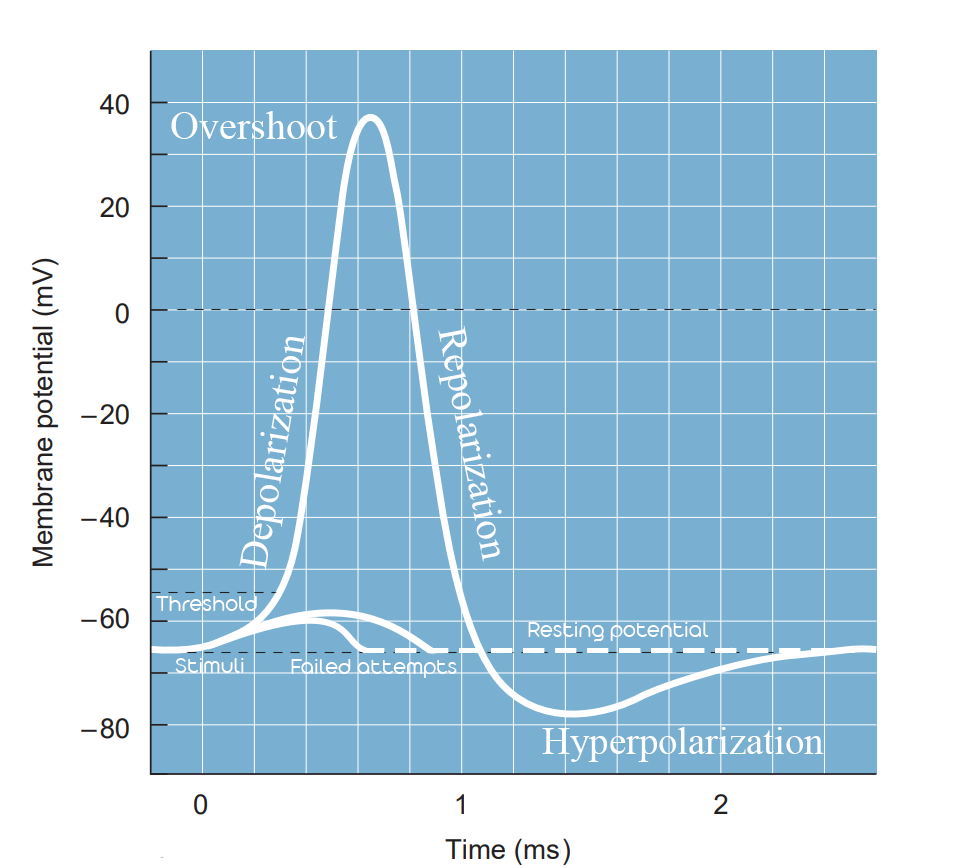
\includegraphics[width=0.6\linewidth]{Pictures/Svet/Untitled-1.png}
  \caption{The action potential spike, indicating the different phases of depolarization, repolarization, and hyperpolarization \cite{wood1996neuroscience}.}\label{fig:AP}
\end{figure}


\subsubsection{ Na\(^+\)dependent depolarization }\label{sec:depol}
%\subsubsection{The \gls{gls:depol} phase of \gls{Na}[-dependent] \gls{ap} results from the transient entry of \gls{Na} \glspl{gls:ion} through \gls{gls:vgate}[d] \gls{Na} channels.}
The threshold for initiation of \gls{Na}[-dependent] action \gls{gls:Pote} is due to \gls{gls:vgate}[d] \gls{Na} channels only opening in response to a \gls{gls:depol} of \qtyrange{-50}{-40}{\mV}, hence the classification `\gls{gls:vgate}[d]' \cite{Hammond2015ch4}. 

%{}\gls{Na} channels are opened by \gls{gls:depol} and once opened, they reinforce the \gls{gls:membrane} \gls{gls:depol} and therefore their own activation: a self-maintained process,\footnotemark~which is why the \gls{Na}[-dependent] \gls{ap} is all or none.\footnotetext{Also commonly refered to as a `positive feedback cycle'.}
%Once initiated, the \gls{ap} propagates along an axon without decaying in amplitude, at rates ranging between \qtyrange{1}{100}{\meter\per\s}. 
%This propagation proceeds without \gls{gls:attenuation} due to the density of \gls{gls:vgate}[d] \gls{Na} channels remains constant along the axon; as well due to the presence of insulating \glspl{gls:myelin}. 
%Once the channels become inactive, they may not reopen, ensuring that \gls{ap} only propagates forward. 
%originaltextend
%The time during which the \gls{Na} channel stays open is the mean open time, denoted \(\tau_o\) \cite{Hammond2015ch4}.\footnote{The letter  `o', not the number `0'}
%The functional significance of this value is the following: during a time equal to \(\tau_o\) the channel has a high probability of staying open. 

The \unit[per-mode = symbol]{\ucur\sodium\per\V} relation is obtained by plotting the amplitude of the unitary current \(\br{\ucur\sodium}\) versus \gls{gls:mPote} \(\br{\unit{\V\membrane}}\). This relation is linear between \qtyrange{-50}{0}{\mV}, as illustrated in \textbf{\Cref{fig:unitcurNa}}. For \glspl{gls:mPote} \gls{gls:hypol} beyond \qty{-50}{\mV}, \(\ucur\sodium\) will have close to no value. As illustrated by \cref{eq:Na}, the \gls{Na} channel has a reduced strength of gradient, drastically lowering the probability of opening \cite{Hammond2015ch4}.\footnote{Quantitative data for \glspl{gls:mPote} more depolarized than \qty{0}{\mV} is, \emph{bizarrely}, lacking.}

%When the activity of a single \gls{Na} channel is recorded at different test \glspl{gls:Pote}, it was observed that the amplitude of the inward unitary current \(\br{\ucur\sodium}\) diminishes proportionately with the state of \gls{gls:membrane} \gls{gls:depol}~\cite{Hammond2015ch4}. 
The critical point of the current/voltage relation is the \gls{gls:mPote} for which the current is zero; i.e. the \gls{gls:rPote} of the current \(\br{\equi\reverse}\) (\textbf{\Cref{fig:unitcurNa}}). 
Because exclusively \gls{Na} \glspl{gls:ion} flow through \gls{Na} channels, the \gls{gls:rPote} is equal to \(\equi\sodium\). 
From \qty{-50}{\mV} to \(\equi\reverse\), \(\ucur\sodium\) is inward and its amplitude decreases. This results from the decrease of the \gls{Na} driving potential \(\br{\unit{\V\membrane}-\equi\sodium}\) as the \gls{gls:membrane} approaches the \gls{gls:rPote} for \gls{Na} \glspl{gls:ion}. 
For \glspl{gls:membrane} \gls{gls:depol} greater than \(\equi\reverse\), \(\ucur\sodium\) is now outward. Above \(\equi\reverse\), the amplitude of the outward \gls{Na} current progressively increases as the driving potential for the exit of \gls{Na} \glspl{gls:ion} increases. 

The relation \unit[per-mode = symbol]{\ucur\sodium\per\V} is \gls{gls:linear}[ly] described by the equation \(\ucur\sodium = \ucon\sodium \br{\unit{\V\membrane}-\equi\sodium}\), where \unit{\V\membrane} is the test potential, \(\equi\sodium\) is the \gls{gls:rPote} of the \gls{Na} current, and \(\ucon\sodium\) is the \gls{gls:admit} of a single \gls{Na} channel (unitary \gls{gls:admit}). The value of \(\ucon\sodium\) is given by the slope of the linear \unit[per-mode = symbol]{\ucur\sodium\per\V} curve (\textbf{\Cref{fig:unitcurNa}}). It has a constant value at any given \gls{gls:mPote}. This value varies between \qtyrange{5}{18}{\pico\siemens} depending on the preparation.

 
The probability of \gls{gls:vgate}[d] \gls{Na} channels opening is dependent on voltage and time. During cell recordings of \gls{Na} channels, observations showing that when the \gls{gls:mPote} depolarizes, the probability of the \gls{Na} channel being in the open state increases proportional to \gls{gls:depol} until reaching a maximal level~\cite{Hammond2015ch4}. 
The greater the \gls{gls:depol}, the higher is the probability of an individual \gls{Na} channel opening. 
Variation also comes from the time, with greater probability of a channel opening towards the start of \gls{gls:depol}.
Additional observations show that after \qtyrange{4}{6}{\ms}, the probability of the \gls{Na} channel being in the open state decreases drastically~\cite{Hammond2015ch4}. 
Even with a large \gls{gls:depol} step: the \gls{Na} channel inactivates after \qtyrange{4}{6}{\ms}~\cite{Hammond2015ch4}. 
%The probability of the \gls{Na} channel being in the open state at time \(t=\qty{2}{\ms}\), for example, increases with the amplitude of the depolarizing step. To generalize, at \qty{-30}{\mV} the open probability is maximum, and the channels inactivate in \qty{4}{\ms}. 

{}\(\curr\sodium\) is the macroscopic current, or the sum of all unitary currents \(\ucur\sodium\) flowing through all the open \gls{Na} channels of the \gls{gls:membrane} being recorded. %Shown in \Cref{fig:unitcurNa}b, an average of \(\num{300}\) unitary \gls{Na} currents elicited by a \gls{gls:depol} pulse of \(\qty{40}{\mV}\). 
For any given potential, the average of inward \gls{gls:flux} for \gls{Na} rises quickly, reaching the peak at time, \(t=\qty{1.5}{\ms}\) \cite{Hammond2015ch4}. 
The peak corresponds to the time when most of the \gls{Na} channels are opened at each trial. 
Subsequently, the average now decays with time because the \gls{Na} channels have a proportionately lower probability of being open.\footnotemark~At each trial, the \gls{Na} channel does not trigger inactivation at exactly the same time, which explains the progressive decay of the average macroscopic \gls{Na} current. 
\footnotetext{Owing to the inactivation of the \gls{Na} channel.}

%The averaged current does not have a rectangular shape because the \gls{Na} channel does not open with the same delay and does not inactivate at the same time at each trial. 


The greater the numerical quantity of \gls{Na} channels opened by \gls{gls:depol}, the smoother the current's sum total \gls{Na} will be. \anakintodo{Should get across the idea that an action potential is a sum of many parts}
The value of \(\curr\sodium\) at each time \(t\) at a given \gls{gls:Pote} is: 
\begin{equation}
  \curr\sodium = p_t \, N \, \ucur\sodium = p_t \sum^N_{n=1} \, \sbr{\ucur\sodium}_n \label{eq:nasum}
\end{equation}
with \(N\) as the total number of \gls{Na} channels in the \gls{gls:membrane} being recorderd and \(p_t\) is the opening probability at time \(t\). 
%\(\ucur\sodium\) is the unitary \gls{Na} current.
%of the \gls{Na} channel; it depends on the \gls{gls:mPote} and on the channel opening and inactivating rate constants. 
%and Np(t) is the number of \gls{Na} channels open at time \(t\). 
Subsequently, the relation of the macroscopic \gls{Na} current \(\curr\sodium\) and voltage \(\unit{\V}\) is not linear, but rather has a recognizable skewed normal distribution, illustrated in \textbf{\Cref{fig:IVdist.}}, with a peak at around \qty{-40}{\mV}. 
%\begin{figure}[H]
 % \centering
  %\includegraphics[width=0.5\textwidth]{Pictures//Anakin/I-%V.bell.png}
  %\caption{The \(\curr\sodium/\unit{\V}\) relation has a bell shape. (From Chiu Sy, ritchie JM, bogart rb, Stagg d (1979) A quantitative description of \gls{gls:membrane} currents from a rabbit myelinated nerve J. Physiol.292, 149–166)}\label{fig:IVdist.}
%\end{figure}
 
For small depolarization steps, the peak amplitude of current is small, \(\br{\qty{0.2}{\nano\ampere}}\), and has a low peaking rate \(\br{\qty{1}{\milli\second}}\)~\cite{Hammond2015ch4}. At these \glspl{gls:Pote}, the \gls{Na} driving potential is strong but the \gls{Na} channels have a low probability of opening. Therefore, \(\curr\sodium\) is small since it represents the current through a small number of open \gls{Na} channels. 

As the depolarizing steps increase in amplitude \(\br{\qtyrange{-42}{-35}{\mV}}\), the amplitude of \(\curr\sodium\) increases to a maximum \(\br{\qty{-3}{\nA}}\) and the time to peak decreases to a minimum \(\br{\qty{0.2}{\ms}}\)~\cite{Hammond2015ch4}. 
Larger \glspl{gls:depol} increase probability of \gls{Na} channels being in the open state and shorten the opening delay. 
Therefore, though the amplitude of \(\ucur\sodium\) decreases by \qtyrange{-63}{-35}{\mV}, the amplitude of \(\curr\sodium\) increases, as a consequence of the increasing quantity of open \gls{Na} channels. 

After the peak, the amplitude of \(\curr\sodium\) decreases to zero, past the peak the probability of opening is no longer enough to compensate for the decrease of \(\ucur\sodium\). 
The \gls{gls:rPote} of \(\curr\sodium\) is the same as that of \(\ucur\sodium\), depending only on the \gls{gls:excell} and \gls{gls:incell} concentrations of \gls{Na} \glspl{gls:ion}.

\(\curr\sodium\) changes polarity for \unit{\V\membrane} more depolarized than Erev: it is now an outward current whose amplitude increases with the \gls{gls:depol} 

\subsubsection{K\(^+\) dependenent repolarization}

In addition to \gls{Na} channel inactivation, the \gls{gls:repol} phase of the \gls{ap} results from \gls{K} channel activation. The \gls{gls:vgate}[d] channels that participate in \gls{gls:membrane} \gls{gls:repol} are so called `delayed rectifiers', which activate after a delay following the \gls{gls:membrane} \gls{gls:depol}~\cite{Hammond2015ch4}. The function of delayed rectifier channels is the transduction of \gls{gls:membrane} \gls{gls:depol} into an outward \gls{gls:flux} of \gls{K} \glspl{gls:ion}, which causes the membrane to repolarize. 

The gating behavior of the delayed rectifier channel is different from that of the \gls{Na} channel. Whereas all four voltage-sensitive domains in \gls{K} channels must be activated in order for pore opening to occur, \gls{Na} channel pore opening requires activation of only three voltage-sensitive domains\cite{Hammond2015ch4}. This is also reflected in the \gls{hh} model, as shall be explained. 


Similar to \gls{Na} channels, both the amplitude of \(\ucur\potassium\) and the time spent by the channel in the open state increase with \gls{gls:depol}. 
The \(\ucur\potassium/\unit{\V}\) relation (\(\ucur\potassium = \ucon\potassium(\unit{\V\membrane}-\equi\potassium\))) is linear between \qtyrange{-50}{20}{\mV}(\textbf{\Cref{fig:rangeThree}}). 

Linear back-extrapolation gives a \gls{gls:rPote} value around \qtyrange{-90}{-80}{\mV}, a value close to \(\equi\potassium\) calculated from the Nernst equation. This means that from \qty{-80}{\mV} to more depolarized \glspl{gls:Pote}, which correspond to the physiological conditions, the \gls{K} current is outward (\textbf{\Cref{fig:rangeThree}}). For more \gls{gls:hypol} \glspl{gls:Pote}, the \gls{K} current is inward. The value of \(\ucon\potassium\) is given by the slope of the linear \(\ucur\potassium/V\)curve. It has a constant value at any given \gls{gls:mPote}. This value varies from \qtyrange{10}{15}{\pico\siemens} depending on the preparation.



The equation for the macroscopic \gls{K} current \(\curr\potassium\)  is analagous to the equation of \(\curr\sodium\) in \Cref{eq:nasum}
\begin{equation}
    \curr\potassium = N p_o \ucur\potassium = p_o \sum^N_{n=1} \, \sbr{\ucur\potassium}_n \label{eq:ksum}
\end{equation}
 The \(\curr\potassium/\unit{\V}\) relation (\textbf{\Cref{fig:Kcurrent}}) shows that the whole cell current varies linearly with voltage from a threshold \gls{gls:Pote} which, for those conditions, is around \qty{-40}{\mV}. When the \gls{gls:membrane} is more \gls{gls:hypol} than the \gls{gls:tPote}, very few channels are open and \(\curr\potassium\) is equal to zero. For \glspl{gls:mPote} more depolarized than the \gls{gls:tPote}, \(\curr\potassium\) depends on \(p_o\) and the driving potential state \(\unit{\V} - \equi\potassium\) which augments with \gls{gls:depol}. Once \(p_o\) is maximal, \(\curr\potassium\) augments linearly with \gls{gls:depol} since it depends only on the driving potential. 

\begin{figure}[H]
\centering
    \begin{subfigure}[t]{0.45\textwidth}
    \centering
    \caption{}\label{fig:unitcurNa}
      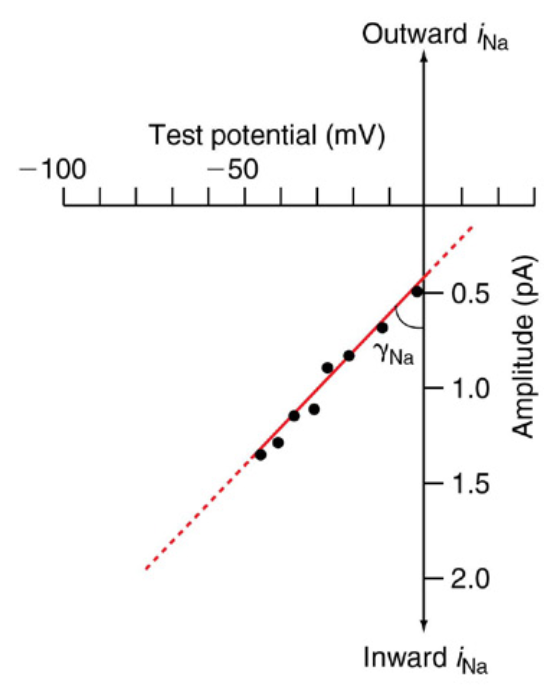
\includegraphics[height=5.5cm]{Pictures/Anakin/iNa-VNa.png}
    \end{subfigure}
    \hfill
    \begin{subfigure}[t]{0.45\textwidth}
    \centering
    \caption{}\label{fig:rangeThree}
      \includegraphics[height=5.5cm]{Pictures/Anakin/I-V.K.png}
    \end{subfigure}

    
     \begin{subfigure}[t]{0.45\textwidth}
    \centering
    \caption{}\label{fig:IVdist.}
      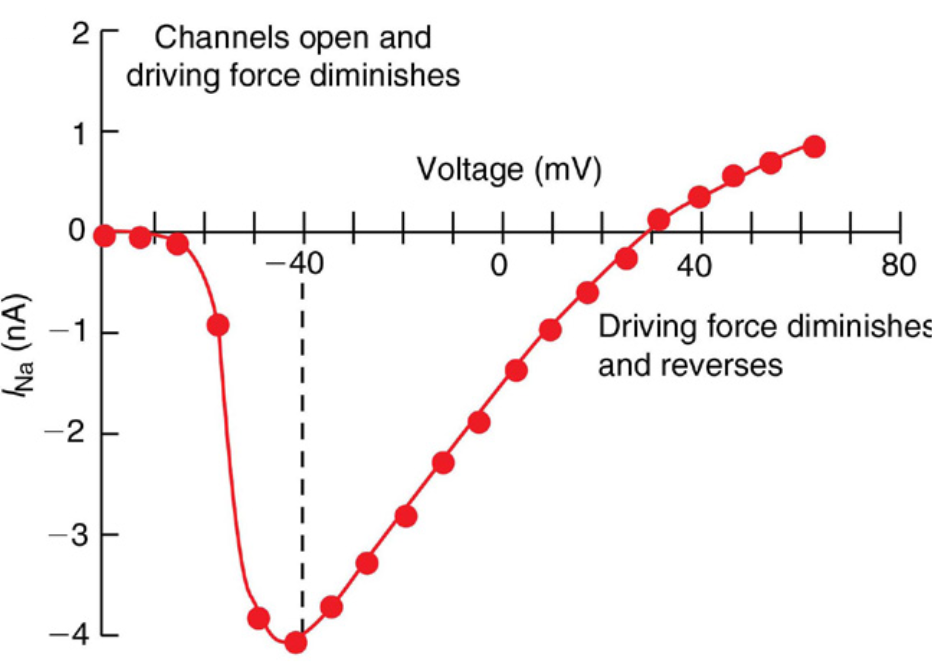
\includegraphics[height=4.5cm]{Pictures/Anakin/I-V.bell.png}
    \end{subfigure}
     \begin{subfigure}[t]{0.45\textwidth}
     \vspace{0.7em}
    \centering
    \caption{}\label{fig:Kcurrent}
      \includegraphics[height=4cm]{Pictures/Anakin/IK-V.png}
    \end{subfigure}
    
      \caption{The relationship of current and voltage: (a) The single-channel \gls{Na} current/voltage \(\br{\unit[per-mode = symbol]{\ucur\sodium\per\volt}}\) relationl (b) The single-channel \gls{K} current/voltage (\(\ucur\potassium\)/V) relation.\(\ucur\potassium\) reverses at =\qty{-75}{\mV} and \(\cond\potassium = \qty{14}{\pico\S}\). (c) Characteristics of the macroscopic \(\curr\sodium/\unit{\V}\) relation; (d) Characteristics of the macroscopic delayed rectifier \gls{K} current. The amplitude of the current at steady state is plotted against test \gls{gls:Pote}. The \gls{gls:Pote} threshold for its activation is \qty{-40}{\mV}. From Hammond 2015 \cite{Hammond2015ch4} }\label{fig:i/I-V}
\end{figure}


To summarize, %owing to their delay of opening, 
delayed rectifier channels begin to open when the \gls{gls:membrane} is has undergone \gls{gls:depol} by the entry of \gls{Na} \glspl{gls:ion} through open \gls{gls:vgate}[d] \gls{Na} channels. 
Therefore, the exit of \gls{K} \glspl{gls:ion} does not occur at the same time as the entry of \gls{Na} \glspl{gls:ion}. This allows the \gls{gls:membrane} to first depolarize in response to the entry of \gls{Na} \glspl{gls:ion} and then to repolarize as a consequence of the exit of \gls{K} \glspl{gls:ion} \cref{fig:Knumber}.
\begin{figure}[H]
    \centering
    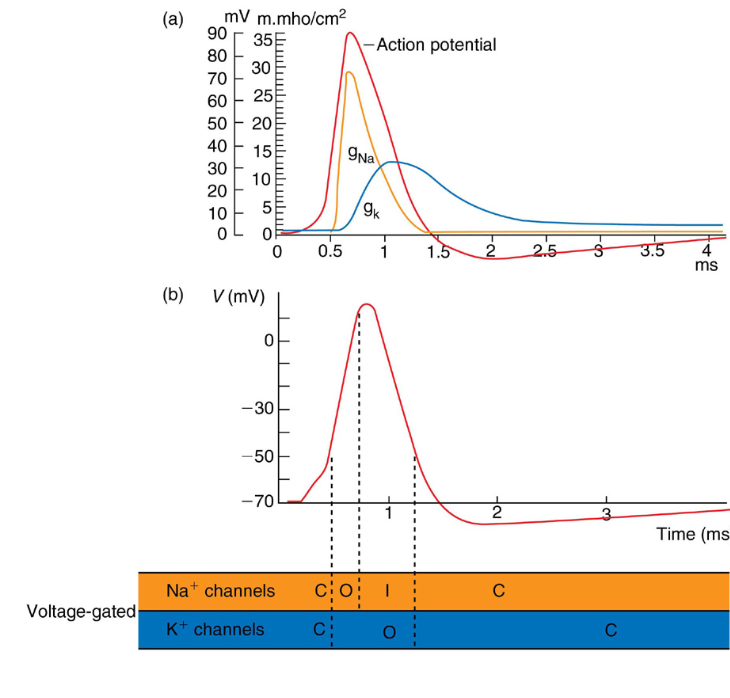
\includegraphics[width=0.8\textwidth]{Pictures//Anakin/N.K.png}
    \caption{Gating of \gls{Na} and \gls{K} channels during the \gls{Na}[-dependent] \gls{ap}.(a) Interpretation of the manner in which the conductances to \gls{Na} and \gls{K} \(\br{\unit{m.mho/cm^2}}\) contribute to the \gls{ap} (\unit{\mV}). (b) State of the \gls{Na} and \gls{K} \gls{gls:vgate}[d] channels during the course of the \gls{ap}. O, channels open; I, channels inactivate; C, channels close or are closed \cite{Hammond2015ch4}}\label{fig:Knumber}
\end{figure}

\end{document}


% \end{document}


% \subsubsection{Activation and inactivation curves}
% The `activation rate' is the rate at which macroscopic current flows in response to a \gls{gls:depol} step. 
% The \gls{Na} current is recorded in voltage clamp mode~\cite{Hammond2015ch4}.
% \footnote{See \Cref{sec:Vclamp}}~Depolarizing steps from \qtyrange{-70}{20}{\mV} are applied from a holding \gls{gls:Pote} of \qty{-80}{\mV}. When the ratio of the peak current at each test \gls{gls:Pote} is compared against the maximal peak current \(\br{\curr\sodium/\curr\sodium{\,}_{max}}\); the activation curve of \(\curr\sodium\) can be visualized \cref{fig:actinact}. 
% %The distribution is fitted, unsurprisingly, by a sigmoidal curve consistent with logistic growth. 
% %In this preparation, the ceiling of \gls{Na} channel activation was measured at \qty{-60}{\mV}. Yet, already at \qty{-40}{\mV}, \(\curr\sodium\) reaches a peak, \(\curr\sodium/\curr\sodium{\,}_{max} = 1\). 
% This steepness of activation is characteristic of \gls{gls:vgate}[d] \gls{Na} channels. 

% An `inactivation rate', comes as a result of a current decaying during a maintained \gls{gls:depol}. 
% %To study inactivation, the \gls{gls:membrane} is held at varying \glspl{gls:Pote} and a fixed \gls{gls:depol} value is applied where \(\curr\sodium\) is maximal (\qty{0}{\mV}, for example). 
% The amplitude of \gls{Na} current plotted against the holding \gls{gls:Pote}, shows that \(\curr\sodium\) begins to inactivate at \qty{-90}{\mV} and is fully inactivated at \qty{-50}{\mV}~\cite{Hammond2015ch4}. 
% %Taking account that the resting \gls{gls:mPote} in this preparation is around \qty{-80}{\mV}, some of the \gls{Na} channels are already inactivated at rest. 
% \begin{figure}[H]
%   \centering
%   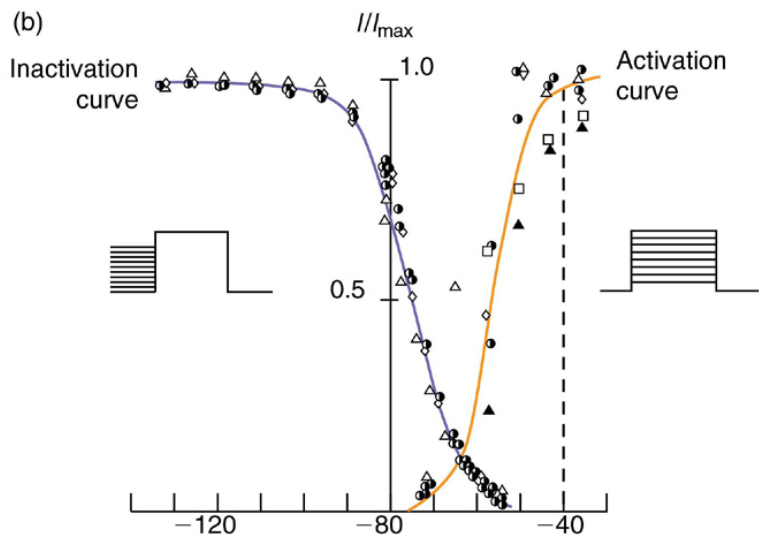
\includegraphics[width=0.5\linewidth]{Pictures//Anakin/activ-inactiv.png}
%   %\caption{Activation (right curve) and inactivation (left curve) curves obtained from nine different experiments. The voltage protocols used are shown in insets. In the ordinates, I/Imax represents the ratio of the peak \gls{Na} current (I) recorded at the tested \gls{gls:Pote} of the abscissae and the maximal peak \gls{Na} current (Imax) recorded in this experiment. (From Chiu Sy, ritchie JM, bogart rb, Stagg d (1979) A quantitative description of \gls{gls:membrane} currents from a rabbit myelinated nerve. J. Physiol.292, 149–166) }\label{fig:actinact}
%   \caption{}\label{fig:actinact}
% \end{figure}



% \subsection{Repolarization the membrane potential}
% %\subsection{The \gls{gls:repol} phase of the \gls{Na}[-dependent] \gls{ap} results from \gls{Na} channel inactivation and partly from \gls{K} channel activation}

% The \gls{gls:repol} phase of the \gls{Na}[-dependent] \gls{ap} results from \gls{Na} channel inactivation and partly from \gls{K} channel activation. The \gls{gls:vgate}[d] channels that participate in \gls{gls:membrane} \gls{gls:repol} are so called `delayed rectifiers', which activate after a delay following the \gls{gls:membrane} \gls{gls:depol} and have a low inactivate rate~\cite{Hammond2015ch4}. The function of delayed rectifier channels is the transduction of \gls{gls:membrane} \gls{gls:depol} into an outward \gls{gls:flux} of \gls{K} \glspl{gls:ion}. 

% % The gating behavior of the delayed rectifier channel is different from that of the \gls{Na} channel. Whereas all four voltage-sensitive domains in \gls{K} channels must be activated in order for pore opening to occur, \gls{Na} channel pore opening requires activation of only three voltage-sensitive domains. 
% % Thus, part of the difference in activation speed between \gls{Na} and \gls{K} channels may be due to the lesser number of voltage-sensitive domains required to move in \gls{Na} channels.

% The mean open time, \(\tau_o\), measured in the clamped patch is \qty{4.6}{\ms}. While the mean closed time, \(\tau_c\), is \qty{1.5}{\ms}, illustrated by \Cref{fig:Kchannel}. As seen in the figure, during a \gls{gls:depol} to \qty{0}{\mV} the delayed rectifier channels spend a greater time in the open state, compared to the closed state: at \qty{0}{\mV} the average probability of channels being open is relatively high \(\br{p_o = 0.76}\)~\cite{Hammond2015ch4}.
% % In order to test whether the delayed rectifier channels show some inactivation, long-lasting recordings are performed. 
% % Though no significant inactivation is apparent during test pulses in the range of seconds, during long test \glspl{gls:depol} (in the range of minutes) the channel shows steady-state inactivation at positive holding \glspl{gls:Pote} (not shown). 
% % Therefore, in the range of seconds, the inactivation of the delayed rectifier channel can be omitted: the channel fluctuates between the closed and open states:
% % \[C\rightleftharpoons O\]
% % The transition from the closed (C) state to the open (O) state is triggered by \gls{gls:membrane} \gls{gls:depol} with a delay. 
% Delayed rectifiers activate over the range of milliseconds. By contrast, the \gls{Na} channels activate in a range of sub-milliseconds. 
% During \gls{gls:membrane} \gls{gls:depol} and \gls{gls:repol}, the \gls{Na} channels will frequently transition between \gls{o} and \gls{c} states. 
% \begin{figure}[H]
%     \centering
%     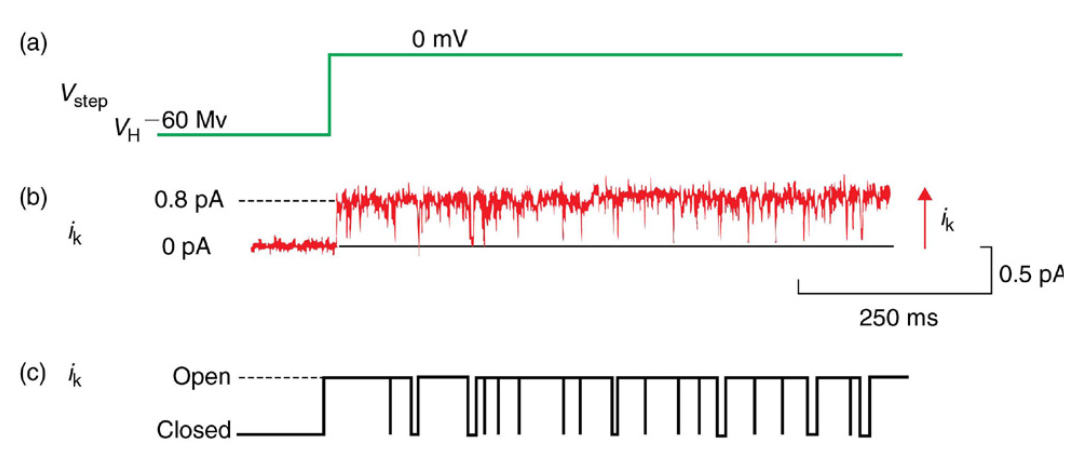
\includegraphics[width=0.8\linewidth]{Pictures//Anakin/Kchannel.png}
%     %\caption{Single \gls{K} channel openings in response to a depolarizing step. The activity of a single delayed rectifier channel expressed from rat brain is recorded in patch clamp (inside-out patch). A depolarizing step to \qty{0}{\mV} from a holding \gls{gls:Pote} of \qty{-60}{\mV}(a) evokes the opening of the channel (b). The elementary current is outward. The channel then closes briefly and reopens several times during the \gls{gls:depol}, as shown in the drawing (c) that interprets the current trace. Adapted from Stühmer W, Stocker M, Sakmann bet al. (1988) potassium channels expressed from rat brain cdNA have delayed rectifier properties. FEBS Lett.242, 199–206, with permission. }\label{fig:rangeThree}
%     \caption{}\label{fig:Kchannel}
%  \end{figure}

% The \gls{K} channel has a constant unitary \gls{gls:admit} \(\br{\ucon\potassium}\)~\cite{Hammond2015ch4}. 
% %In \Cref{fig:rangeThree}a, unitary \gls{K} currents are shown responding to increasing \gls{gls:depol} of \qtyrange{-50}{20}{\mV} from the holding \gls{gls:Pote} of \qty{-80}{\mV}. 
% %It can be observed that both the amplitude of \(\ucur\potassium\) and the time spent by the channel in the open state increase with \gls{gls:depol}. 
% When the mean amplitude of the unitary \gls{K} current is plotted versus \gls{gls:membrane} test potential, a linear \(\ucur\potassium/\unit{\V}\) relation is obtained. This linear \(\ucur\potassium/\unit{\V}\) relation (between \qtyrange{-50}{20}{\mV}) is described by the equation \(\ucur\potassium = \ucon\potassium(\unit{\V\membrane}-\equi\potassium)\), where \unit{\V\membrane} is the \gls{gls:mPote}, \(\equi\potassium\) is the \gls{gls:rPote} of the \gls{K} current, and \(\ucon\potassium\) is the \gls{gls:admit} of the single delayed rectifier \gls{K} channel, which defines the unitary \gls{gls:admit}. 

%Linear back-extrapolation gives a \gls{gls:rPote} value around \qtyrange{-90}{-80}{\mV}, a value close to \(\equi\potassium\) calculated from the Nernst equation. This means that from \qty{-80}{\mV} to more depolarized \glspl{gls:Pote}, which correspond to the physiological conditions, the \gls{K} current is outward. For more \gls{gls:hypol} \glspl{gls:Pote}, the \gls{K} current is inward. The value of \(\ucon\potassium\) is given by the slope of the linear \(\ucur\potassium/V\)curve. It has a constant value at any given \gls{gls:mPote}. This value varies from \qtyrange{10}{15}{\pico\siemens} depending on the preparation. 

% \begin{figure}[H]
%     \centering
%     \includegraphics[width=0.8\textwidth]{Pictures//Anakin/I-V.K.png}
%     %\caption{The single-channel current/voltage (\(\ucur\potassium\)/V) relation is linear.delayed rectifier \gls{K} channels from rat brain are expressed in a myoblast cell line. (a) The activity of a single channel is recorded in patch clamp (cell-attached patch). Unitary currents are recorded at different test \glspl{gls:Pote} (from \qty{-50}{\mV} to \qty{20}{\mV}) from a holding \gls{gls:Pote} at \qty{-80}{\mV}. Bottom trace is the voltage trace. (b)\(\ucur\potassium\)-V relation obtained by plotting the mean amplitude of \(\ucur\potassium\) at the different test \glspl{gls:Pote} tested. \(\ucur\potassium\) reverses at =\qty{-75}{\mV} and gK=14pS. Adapted from Koren G, liman er, logothetis deet al. (1990) Gating mechanism of a cloned potassium channel expressed in frog oocytes and mammalian cells. Neuron2, 39–51.}\label{fig:rangeThree}
%     \caption{}\label{fig:rangeThree}
% \end{figure} 

% The macroscopic delayed rectifier \gls{K}current \(\br{\curr\potassium}\) has a delayed voltage dependence of activation and inactivates within tens of seconds. 
% %Whole cell currents start to activate at \glspl{gls:Pote} positive to \qty{-30}{\mV} and their amplitude is clearly voltage dependent. 
% %When unitary currents recorded from 70 successive depolarizing steps to \qty{0}{\mV} are averaged (Figure4.20b), the macroscopic outward current obtained has a slow time to peak \(\br{\qty{4}{\ms}}\) and lasts the entire depolarizing step. 
% The whole cell current amplitude at steady-state for a given \gls{gls:Pote} is:


% where \(N\) is the number of delayed rectifier channels in the \gls{gls:membrane} recorded, \(p_o\) the open probability at steady state and \(\ucur\potassium\) the elementary current. The number of open channels \(N\,p_o\) increases with \gls{gls:depol} (to a maximal value) and so does \(\curr\potassium\). 

% The \(\curr\potassium/\unit{\V}\) relation shows that the whole cell current varies linearly with voltage from a threshold \gls{gls:Pote} which, for those conditions, is around \qty{-40}{\mV}. When the \gls{gls:membrane} is more \gls{gls:hypol} than the \gls{gls:tPote}, very few channels are open and \(\curr\potassium\) is equal to zero. For \glspl{gls:mPote} more depolarized than the \gls{gls:tPote}, \(\curr\potassium\) depends on \(p_o\) and the driving potential state \(\unit{\V} - \equi\potassium\) which augments with \gls{gls:depol}. Once \(p_o\) is maximal, \(\curr\potassium\) augments linearly with \gls{gls:depol} since it depends only on the driving potential. 
% \begin{figure}[H]
%     \centering
%     \includegraphics[width=0.4\linewidth]{Pictures//Anakin/IK-V.png}
%     %\caption{Characteristics of the macroscopic delayed recti-fier \gls{K} current. The amplitude of the current at steady state is plotted against test \gls{gls:Pote}. The \gls{gls:Pote} threshold for its activation is \qty{-40}{\mV}. From Stühmer W, Stocker M, Sakmann bet al. (1988) potassium channels expressed from rat brain cdNA have delayed rectifier properties. FEBS Lett.242, 199–206. }\label{fig:Kcurrent}
%     \caption{}\label{fig:Kcurrent}
% \end{figure}

% To summarize, %owing to their delay of opening, 
% delayed rectifier channels begin to open when the \gls{gls:membrane} is has undergone \gls{gls:depol} by the entry of \gls{Na} \glspl{gls:ion} through open \gls{gls:vgate}[d] \gls{Na} channels. 
% Therefore, the exit of \gls{K} \glspl{gls:ion} does not occur at the same time as the entry of \gls{Na} \glspl{gls:ion}. This allows the \gls{gls:membrane} to first depolarize in response to the entry of \gls{Na} \glspl{gls:ion} and then to repolarize as a consequence of the exit of \gls{K} \glspl{gls:ion}.
% \begin{figure}[H]
%     \centering
%     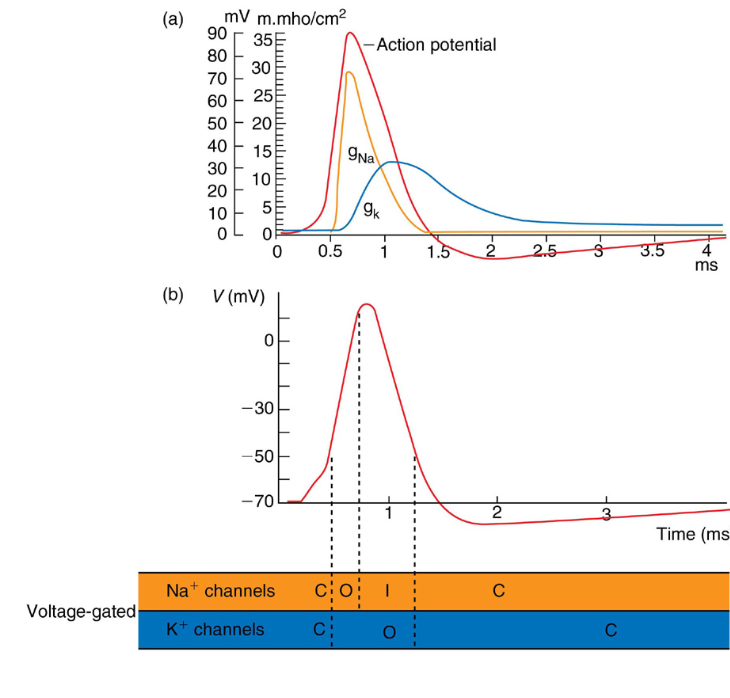
\includegraphics[width=0.8\textwidth]{Pictures//Anakin/N.K.png}
%     %\caption{Gating of \gls{Na} and \gls{K} channels during the \gls{Na}[-dependent] \gls{ap}.(a) Interpretation of the manner in which the conductances to \gls{Na} and \gls{K} contribute to the \gls{ap}. (b) State of the \gls{Na} and \gls{K} \gls{gls:vgate}[d] channels during the course of the \gls{ap}. O, channels open; I, channels inactivate; C, channels close or are closed. Trace (a) adapted from Hodgkin Al, Huxley AF (1952) A quantitative description of \gls{gls:membrane} current and its application to conduction and excitation in nerve. J. Physiol.117, 500–544.}\label{fig:Knumber}
%     \caption{}\label{fig:Knumber}
% \end{figure}



 